\section{Methodology}
The design considerations will be explored in this section. There will also be a full description of how the smart fan system will be implemented. Figure \ref{fig:architecture} shows the basic architecture of the system. Because it is part of a larger modular system, its integration should be seamless. There are basically two modules:

\begin{itemize}
\item The smart fan
\item The sensor node
\end{itemize}

\begin{figure}[h]
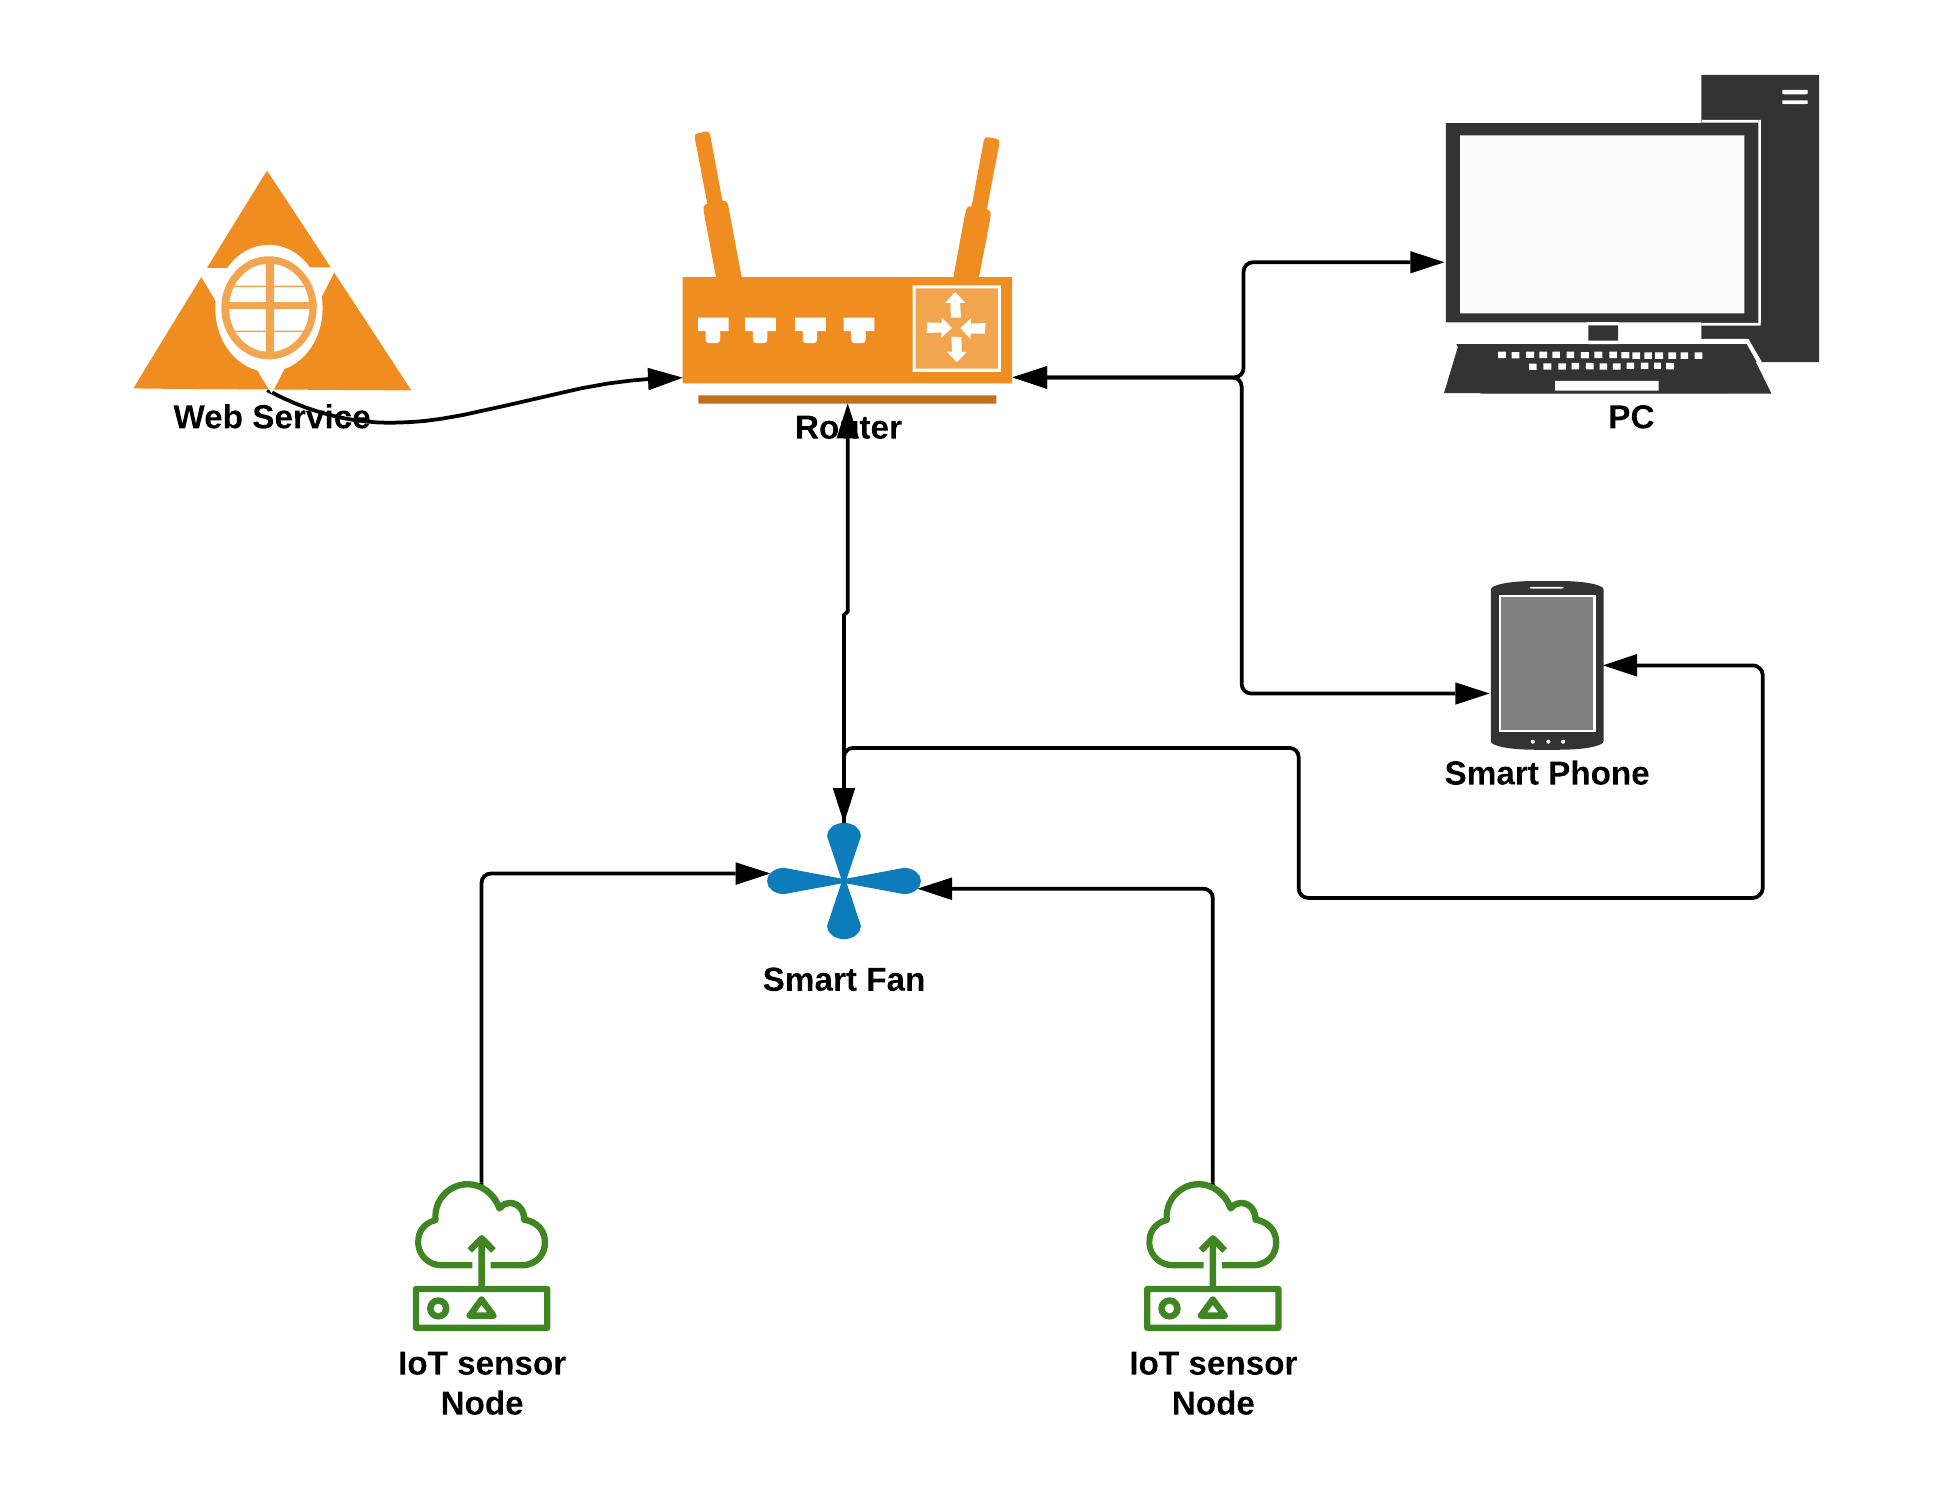
\includegraphics[scale=0.15]{architecture}
\centering
\caption{Design architecture}
\label{fig:architecture}
\end{figure}

The sensor nodes measure the temperature of the room and send it to the smart fan main controller. The sensor nodes are positioned far from the smart fan but in the same room to measure the temperature endpoint after the air has travelled from the smart fan.
\par
The smart fan has the main controller. This controller controls the stepper motor which controls the position of the fan. It also controls the brushless \ac{DC} motor which controls the spinning of the fan. The main controller communicates with sensor nodes via \ac{BLE} then communicates with your device through the \ac{Wi-Fi} router in your home or you can connect to its \ac{Wi-Fi} network.
\par
The following modules break down the design problem:

\subsection{Interface module}

The interface module is responsible for the following:
\begin{itemize}
\item Human-machine interface.
\item Manual overriding of settings and configurations.
\item Creating a visual appeal of the product.
\end{itemize}

The following considerations were made during the design of the interface of the mechanism:
\begin{itemize}
\item Fulfilling the function to control the smart fan remotely.
\item Unlocking the full functionality of the smart fan
\item Ease of use of the interface.
\item Ease of integration with third-party mobile \ac{IoT} applications.
\item Availability on both Android and Web platforms.
\end{itemize}

The interface for this design is intended to be a web and android based application to be installed on the device of the home user. In tandem, it will provide a few buttons to start and stop. This will be crucial to our development as we will provide the user with the ultimate user experience for both advanced and novel users.
The \ac{UX} is a phrase that is strongly related to the \ac{UI}. The distinction between the two is that \ac{UI} is concerned with what a user sees and interacts with, whereas \ac{UX} is concerned with the total experience a user has with a product. It comprises the website, application, hardware packing, and installation, among other things.
\par
The user can receive automatic notifications if they have a web or Android application. In \ac{IoT} applications, the most common scenario is that we want to be notified or alerted if something strange occurs. The user will also be able to keep a proactive eye on the data. The user will undoubtedly be able to control the system remotely as a result of this. This might also be done automatically by the application, based on the instructions provided.

\subsection{Communication module}

The communication module is responsible for the following:

\begin{itemize}
\item Transmitting data from our sensor nodes to the smart fan.
\item Transmitting data from our smart fan to the mobile phone and vice versa.
\item Sending analytics data back to our backend server.
\end{itemize}

The following considerations were made during the design of the interface of the mechanism:

\begin{itemize}
\item Communication must be done over low energy.
\item Communication must be secured with encryption.
\item Communication must be done wirelessly either through \ac{BLE} or \ac{Wi-Fi}.
\end{itemize}

The four most prevalent wireless technologies, \ac{BLE}, \ac{UWB}, ZigBee, and \ac{Wi-Fi}, will be evaluated quantitatively in terms of transmission time, data coding efficiency, protocol complexity, and power consumption in this paper. Network protocol appropriateness is heavily influenced by practical applications but based on existing data, the best technology to be used will be \ac{BLE} Low Energy based on its low consumption power, availability and low overhead.
\par
For communication with the mobile device, \ac{Wi-Fi} will be the appropriate medium. This is based on research that most home users use \ac{Wi-Fi} within their homes and also most of them keep their \ac{Wi-Fi} on connect compared to \ac{BLE} \cite{shimray_use_2019}.
\par
\ac{UART} communication will be used for communication with the \ac{BLE} module. A \ac{UART} provides a bi-directional byte stream so that both ends of a connection can transmit and receive bytes with each other \cite{noauthor_uart_2015}.

\subsection{Software and Processors module}

The software and processing module is responsible for the following:

\begin{itemize}
\item Process information from the interface to actuate it.
\item Control the smart fan.
\item Transmit data to the backend server.
\item Receive data from the sensor nodes.
\item Be able to utilize deep sleep
\item Minimum of 1 \ac{PWM} and \ac{UART} communication pins
\item \ac{Wi-Fi} and \ac{BLE} enabled
\end{itemize}

The following considerations were made during the design of the software and processing module of the mechanism:

\begin{itemize}
\item Computationally less intensive method
\item Secure all communications
\item Low cost of the processors module with \ac{Wi-Fi} and BLE modules
\end{itemize}

Figure \ref{fig:softwarelogic} shows the basic software logic of how the smart fan control module will operate.

\begin{figure}[t]
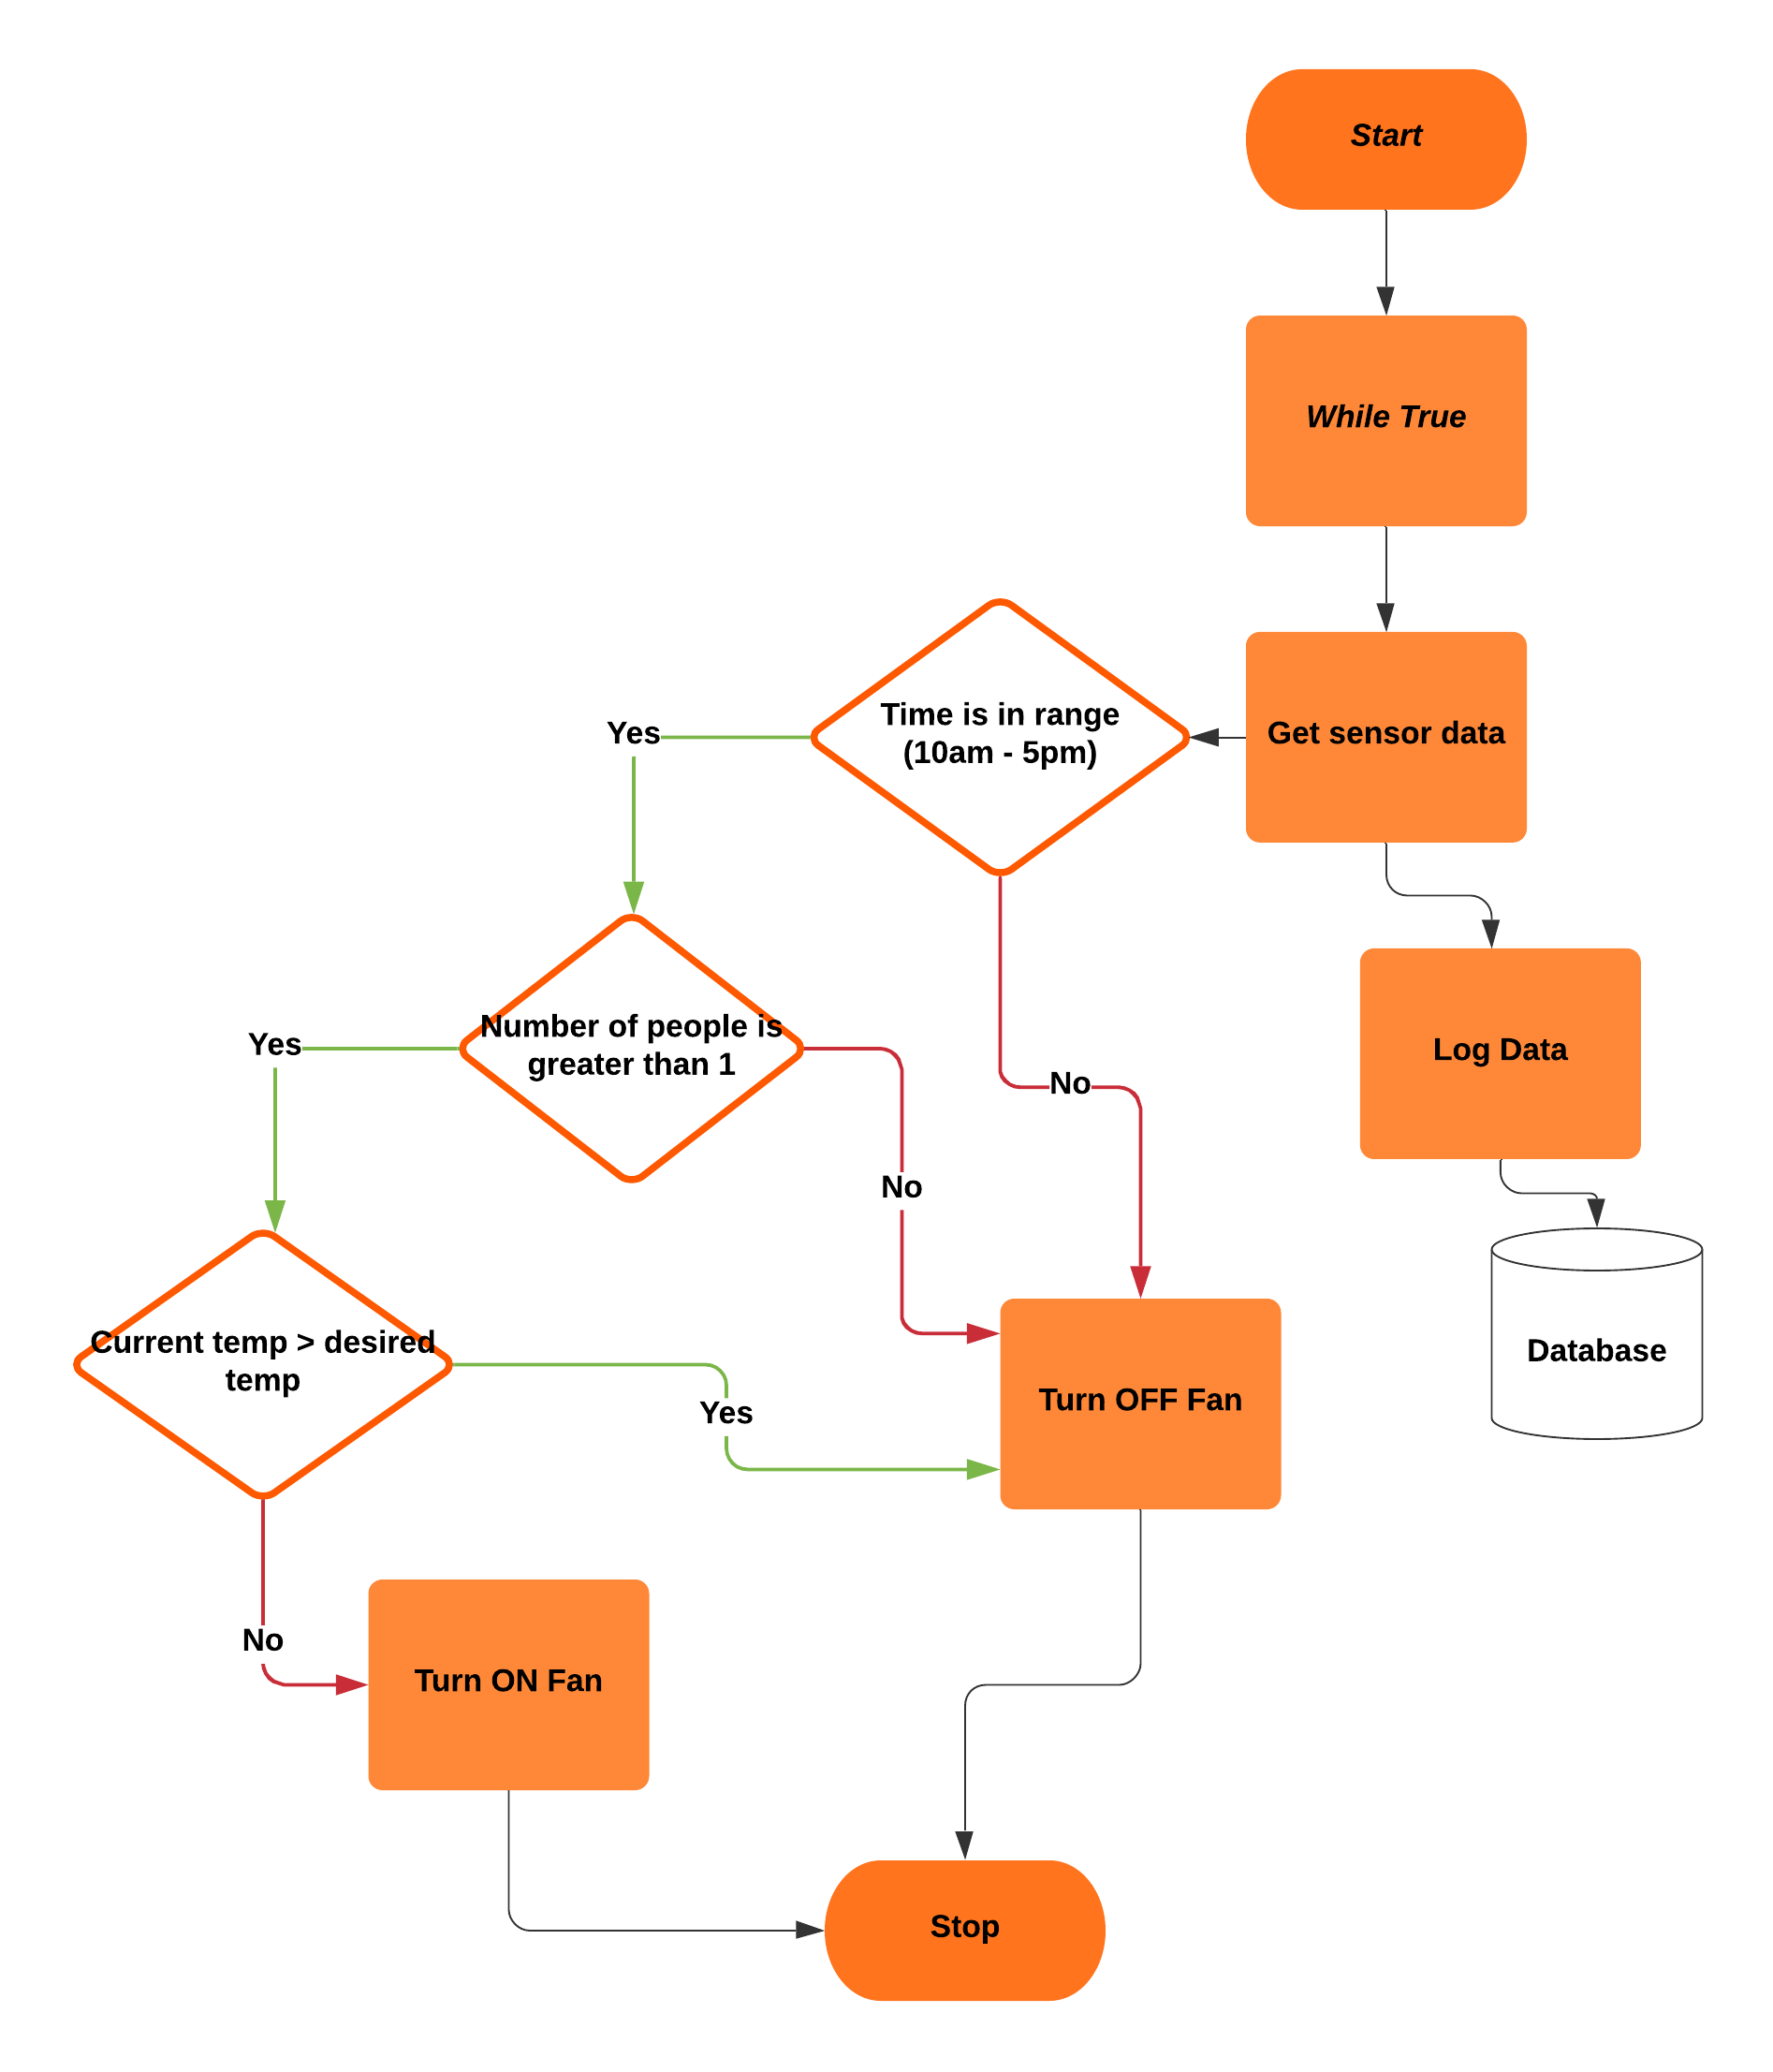
\includegraphics[scale=0.15]{Figures/logic.png}
\centering
\caption{Software Logic}
\label{fig:softwarelogic}
\end{figure}

\subsection{Measurement module}

The interface module is responsible for the following:
\begin{itemize}
\item Measure temperature and humidity.
\item Identify the occupants in the house.
\end{itemize}

The following considerations were made during the design of the measurement module of the mechanism:
\begin{itemize}
\item Fulfilling the function to control the smart fan remotely.
\item Unlocking the full functionality of the smart fan.
\item Ease of use of the interface.
\end{itemize}

\subsection{Actuation module}

The actuation module is responsible for the following:

\begin{itemize}
\item Rotating the Brushless \ac{DC} motor.
\item Rotating the Stepper Motor.
\end{itemize}


\subsection{Assembly module}

The assembly module is responsible for the following:
\begin{itemize}
\item Synergistic integration of the motor and fan blades.
\item Full working of the sensor nodes.
\item Hold the fan up high and maintain its weight.
\end{itemize}

The following considerations were made during the design of the assembly of the mechanism:
\begin{itemize}
\item Use as many modular parts as possible.
\item Using easily available material from the workshops.
\item Must hold the frame so as not to fall.
\end{itemize}

The fan will be assembled by mountain the fan blades on the motor shaft. The fan casing will be added onto the fan blades, while the motor is added into the motor casing. This will be assembled to the stand so as to hold it above. The stand will have an aluminium tube and a base plate to increase stability.
\par
The fan blades will be constructed from a \ac{PVC} tube. The tube will be cut and straightened out after which the blades with equal dimensions will be cut out and rolled to have a curvature. This is to reduce the air resistance as the fan is moving. The blades will be attached to the centre case which will be attached to the motor shaft.
\par
The fan case will be made from small steel wires welded together. It will be moulded into a punched shape and mounted to the motor mount as the fan will be inside the case.
\par
The stand, made from a steel tube, will be joined to the motor mount, hence holding the fan in position. 
\par
For the sensor node, the \ac{PCB} circuitry will be assembled inside the sensor box which will be \ac{3D} printed. A battery will be added to provide power to the sensor node. 

\subsection{Environment module}

The environment module is responsible for the following:

\begin{itemize}
\item Interaction with the environment.
\item Blow maximum air through the inlet diffuser
\end{itemize}

The following considerations were made during the design of the environment module of the mechanism:
\begin{itemize}
\item To minimise noise produced by the fan as it moves.
\item Not to interfere with most of the user’s space
\item Ultimately reduce energy consumption hence helping reduce climate change at large.
\end{itemize}

For the design, the motor should produce the minimum noise possible while rotating. Its aesthetics will be improved by applying paint which will increase the product appeal to the user.
The sensor nodes will also interact with the environment, getting temperature readings from it. The sensor node will be as small as possible and not interfere with the aesthetics of the room.














